\begin{figure}[t]
\centering
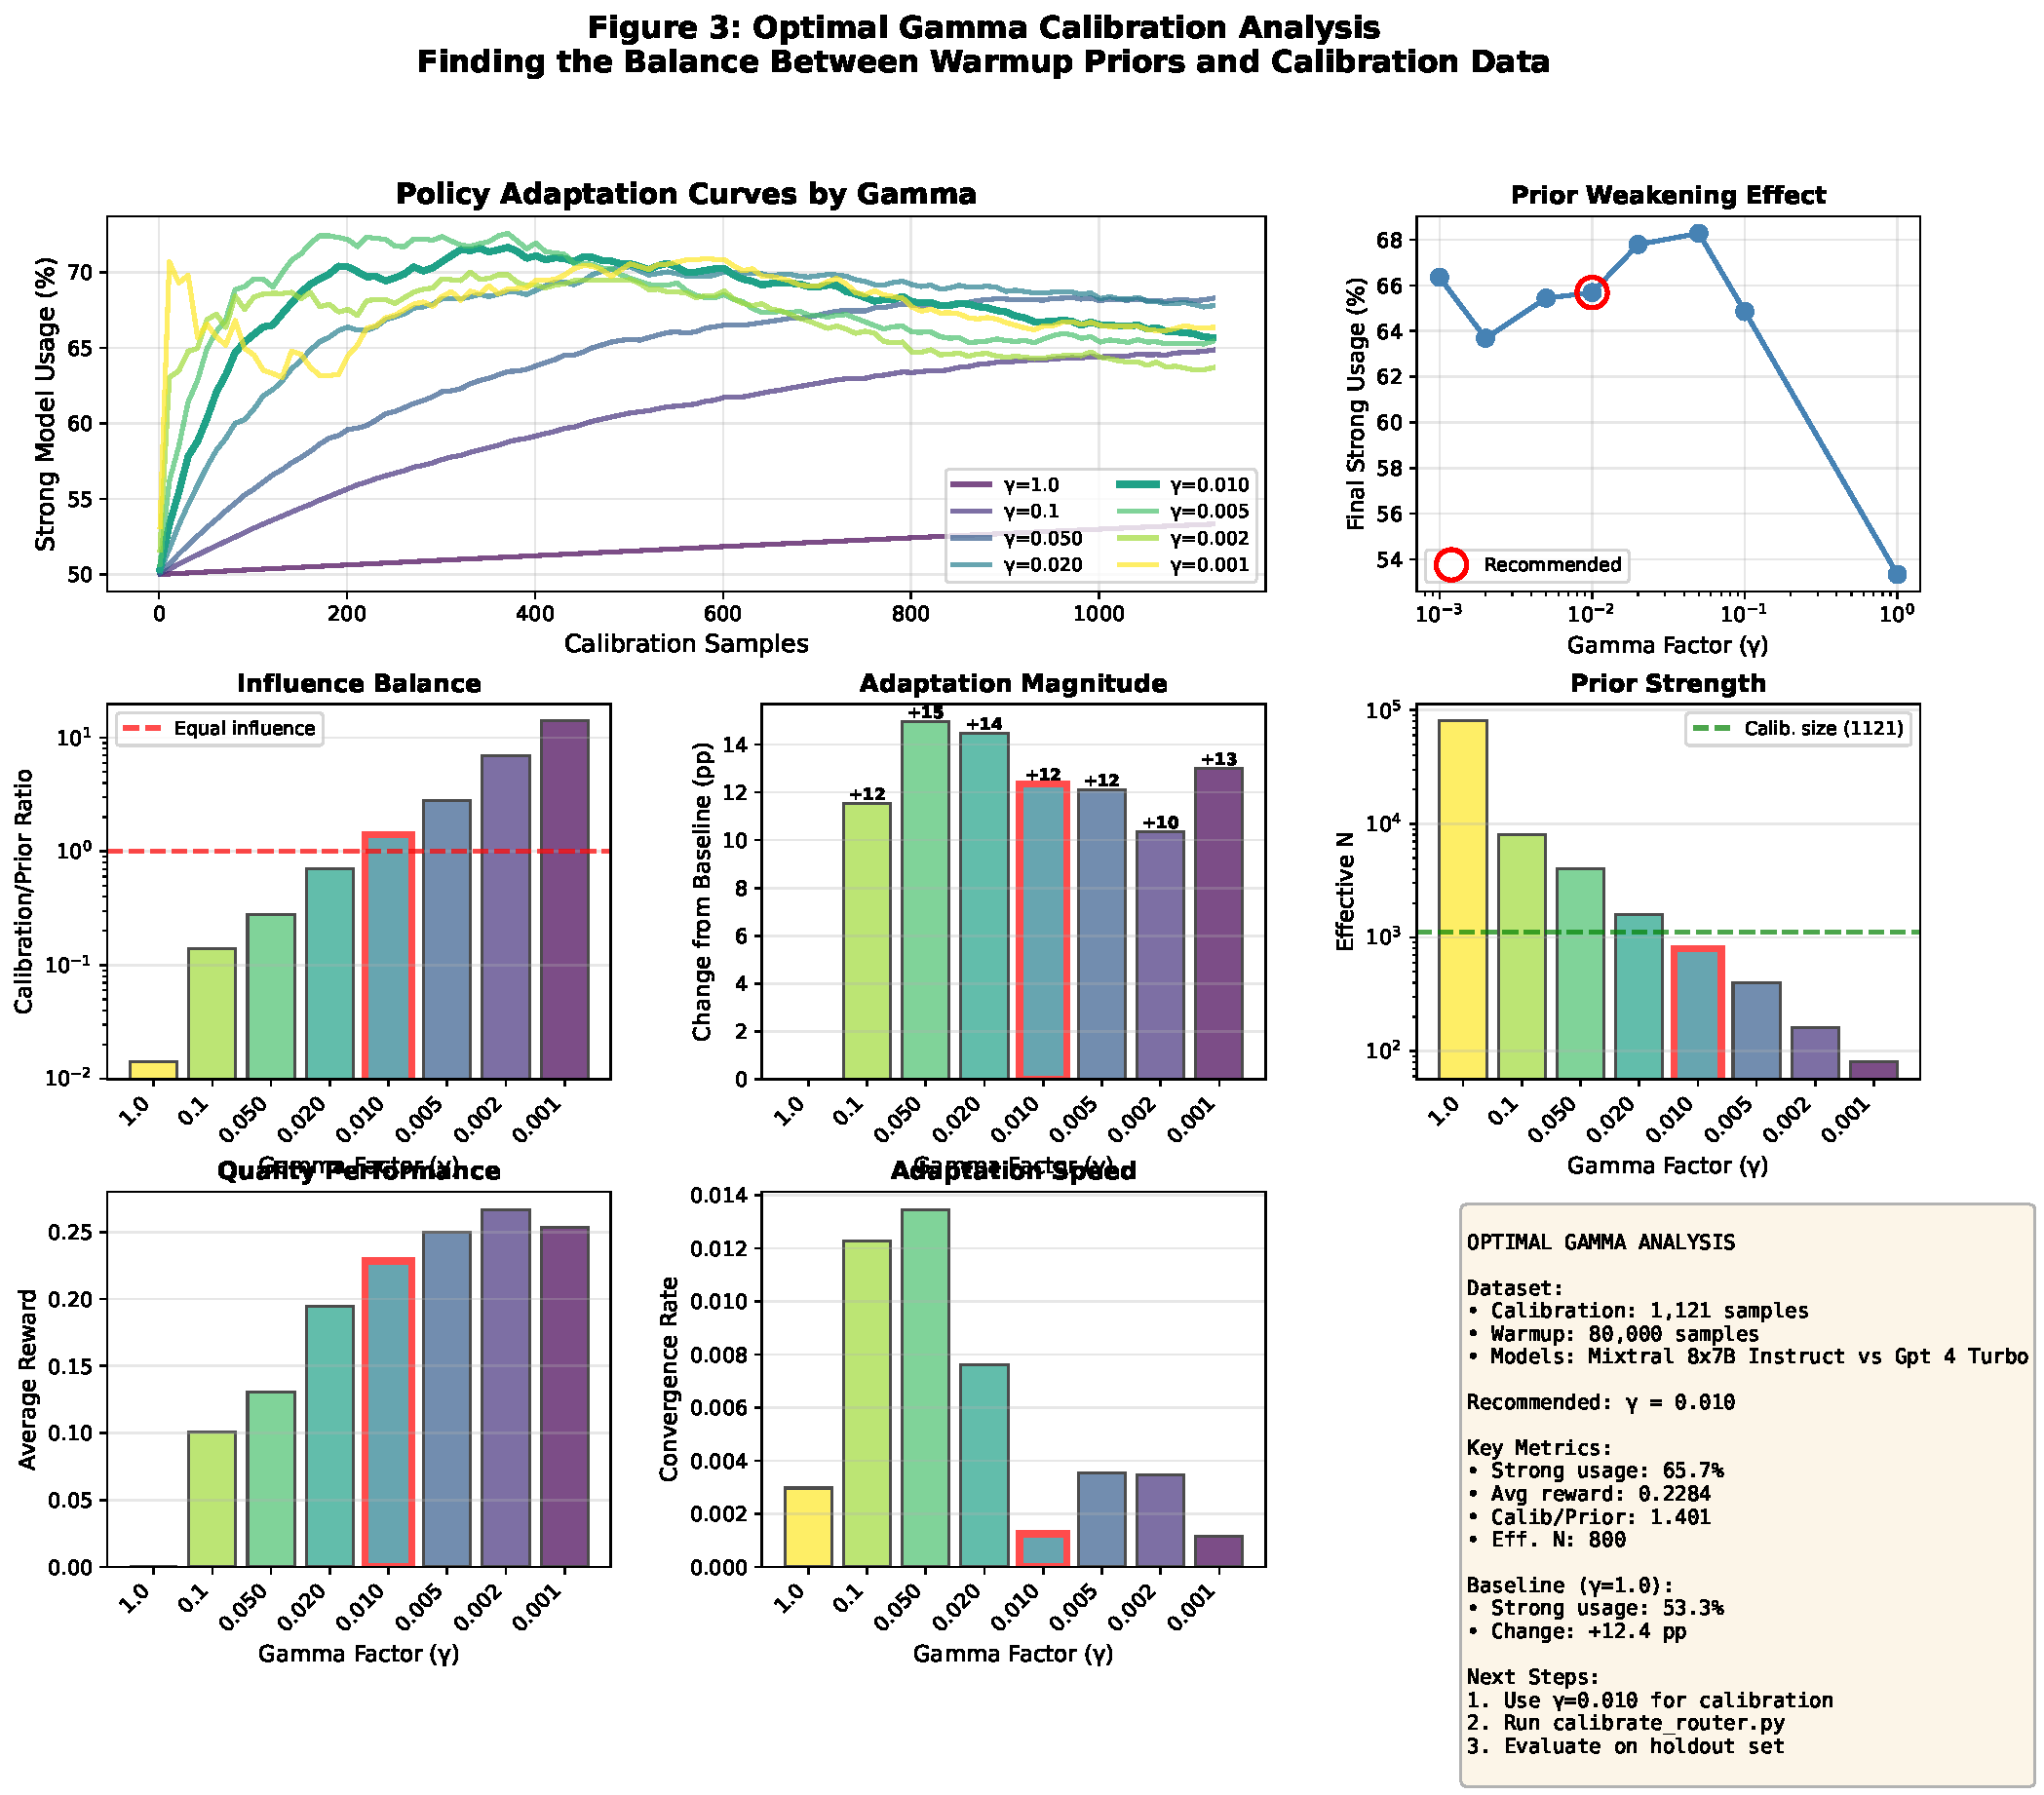
\includegraphics[width=\textwidth]{experiments_v1/03_figure/results/optimal_gamma_analysis.pdf}
\caption{%
\textbf{Optimal Gamma Calibration Analysis with 32-Component PCA.}
We systematically evaluate 8 gamma values to determine the optimal covariance inflation factor for domain adaptation.
The router uses 80,000 warmup samples (corrected RouteLLM data where GPT-4-Turbo wins 68.6\% vs Mixtral's 9.3\%) with 32-component PCA (35.14\% variance) and 1,121 calibration samples.
\textbf{(Top-left)} Policy adaptation curves show how different gamma values affect convergence speed and final routing strategy.
\textbf{(Top-center)} Prior weakening effect demonstrates the relationship between gamma and final strong model usage (baseline: 53.3\% at $\gamma=1.0$).
\textbf{(Top-right)} Influence balance quantifies the Calibration/Prior ratio, with values near 1.0 indicating balanced influence.
\textbf{(Middle row)} Adaptation magnitude, prior strength, and quality performance across gamma values.
\textbf{(Bottom row)} Convergence rate analysis and summary statistics.
The recommended gamma ($\gamma=0.010$, highlighted in red) achieves a Calibration/Prior ratio of 1.401, enabling 1,121 calibration samples to effectively adapt 80,000 warmup priors (effective N = 800).
This results in a 12.4 percentage point increase in GPT-4 usage (from 53.3\% to 65.7\%) while achieving 0.2284 average reward.
The 32-component PCA provides better semantic representation (+6.14\% variance) compared to 23 components, enabling more nuanced routing decisions.
}
\label{fig:optimal_gamma}
\end{figure}
